\documentclass[a4paper,10pt]{article}
\usepackage{paper-en}
\usepackage{hyperref}

\def\thetitle{Shadow isoperimetry}
\def\theauthors{}

\hypersetup{colorlinks=true,
citecolor=black,
linkcolor=black,
anchorcolor=black,
filecolor=black,
menucolor=black,
urlcolor=black,
pdftitle={\thetitle},
pdfauthor={\theauthors}
}
\begin{document}

\title{\thetitle}
\author{\theauthors}
\date{}
\maketitle

\begin{abstract}
We outline a proof of the isoperimetric inequality for Favard area.
\end{abstract}

\section{Introduction}

Given a compact subset $K\subset \RR^n$ let us denote by $a(K)$ its \emph{Favard area}; that is, the average of the areas of orthogonal projections of $K$ onto hyperplanes.
\emph{Area} here means the Lebesgue measures of dimension $n-1$ or the $(n-1)$th Hausdorff measure in dimension $n$, \emph{volume} means the Lebesgue measure in dimension $n$.%
\footnote{This definition agrees with ``Favard length'', but Burago--Zalgaller define ``Favard measure'' with mulitplicity, so it is closer to integralgeometric measure --- maybe it is better to avoid this term? Maybe ``mean shadow area''?}

\begin{thm}{Theorem}\label{thm:main}
Let $K\subset \RR^n$ be a compact subset and let $B\subset \RR^n$ be a ball.
Then
\[
a(K)= a(B)\quad\Rightarrow\quad \vol K\le \vol B.
\]
Moreover, if equality holds, then $K$ contains a congruent copy $B$ and the remaining part has vanishing volume.
\end{thm}

\begin{wrapfigure}{r}{43 mm}
\vskip-4mm
\centering
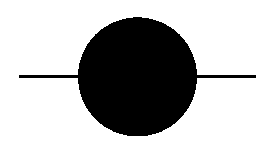
\includegraphics{mppics/pic-10}
\end{wrapfigure}

By a Crofton-like argument \cite[3.3.13]{federer}, this theorem gives a more exact version of the standard isoperimetric inequality.
For the equality case, we gave only a necessary condition, which is not sufficient; an example can be guessed from the picture.
On the other hand, equality holds for the union of a ball with any set of vanishing Favard area,
but these are not the only examples; the latter follows from the result of Kenneth Falconer \cite[Theorem 5.1]{falconer}.

In the proof we adapt an idea of Frederick Almgren, \cite[pp. 454--455]{almgren-1986}.

\begin{thm}{Corollary}\label{cor:borel}
Let $E\subset \RR^n$ be a Borel subset and let $B\subset \RR^n$ be a ball.
Then
\[
\vol E= \vol B \Rightarrow a(E)\ge a(B).
\]
\end{thm}

The equality case in Corollary~\ref{cor:borel} seems harder to characterize, so we do not discuss it here.

Note that $a(E)$ is well-defined for Borel sets. Consider the Borel set
\[
\widetilde E = \{(x,R)\in \RR^n\times \mathrm{O}(n)\ |\ R(x)\in E\}.
\]
The $a(E)$ can be defined as the measure of the projection of $\widetilde E$ to $\RR^{n-1}\times \mathrm{O}(n)$, assuming the normed Haar measure on $\mathrm{O}(n)$. By Suslin's theorem (see~\cite[Section~1.10]{bogachev-i}) a projection of a Borel set is Lebesgue measurable, so $a(E)$ is well defined.

Favard length of various irregular sets has been intensively studied in the last years; see, e.g., \cite{Laba2012,Damian2024}. The isoperimetric problem for Favard length or area has optical and mechanical interpretations originating from Newton's problem of least resistance.

Namely, suppose that there is a body (that is, a set, not necessarily connected, with a piecewise smooth boundary) on the plane with {\it absolutely black} surface. We want to deform it, without changing its area, so as to make its visibility as small as possible. The visibility of a body is the average value of its orthogonal projections to all possible straight lines, that is, the Favard length.

There is another, much more difficult, problem related to minimizing the visibility of a planar body with fixed area and {\it mirror surface}; the so-called problem of {\it camouflaging in billiards}. At present, only below estimates for this value are found; see \cite{cam1,cam2}. Additionally, it is known how to construct a body invisible in $n$ directions $(n=1,\,2,\ldots)$, provided that the angles between them are multiples of $\pi/n$ \cite{invisNpoints}. Some other results are known about invisibility in several directions or from several points in $\RRR^2$ and $\RRR^3$ \cite{book2012,fractal,invis2points}.

The mechanical interpretation, going back to I. Newton \cite{N}, is as follows. A body moves in a rarefied medium of point particles on the plane and rotates very slowly and uniformly. The medium is so rare that mutual interaction of the particles can be neglected. One is interested in minimizing the time averaged value of the force of resistance of the medium. If the body-particle collisions are completely inelastic, so that each particle, after the collision, loses its relative velocity and remains forever near the body, the problem is reduced to the isoperimetric problem for Favard length. If, on the contrary, the collisions are perfectly elastic then the problem amounts to camouflaging in billiards (see, e.g., \cite{book2012}).

\section{Proofs}

Given a compact set $K$, consider the ball $B$ such that $a(K)=a(B)$.
Let us denote by $\kappa=\kappa(K)$ the normal curvature of $\partial B$, so $\tfrac1\kappa$ is the radius of $B$ and
\[
\frac{\omega_{n-1}}{\kappa^{n-1}}=a(K)=a(B),\quad \frac{\omega_{n}}{\kappa^{n}}=\vol B,
\]
where $\omega_n$ is the volume of the unit ball in $\RR^n$.

\begin{thm}{Lemma}\label{lem:support}
Let $K$ be a compact set in $\RR^n$.
Given $\eps>0$, there is a strictly convex body $C$ with smooth boundary such that $C\supset K$,
$\partial C\cap K$ contains a single point, say $p$,
and the mean curvature of $\partial C$ at $p$ is at least $(n-1)\cdot (\kappa(K)-\eps)$.
Moreover, the same holds for some $\eps<0$ unless $\partial K\supset \partial(\conv K)$ or $\vol K=0$;
here $\conv K$ denotes the convex hull of $K$.
\end{thm}

\begin{proof}[Proof for $\eps>0$]
Let us denote by $K_s$ the closed $s$-neighborhood of $K$.
Good thing about $K_s$ is that the convex hull $\conv K_s$ has $C^{1,1}$-smooth boundary; in particular, its second derivatives exist almost everywhere and are bounded.
So the shape operator ($\Shape$), the Gauss curvature $G=\det(\Shape)$, and mean curvature $H=\tr(\Shape)$ are defined almost everywhere on $\partial(\conv K_s)$.
Note also that any hyperplane projection of $K_s$ is the closed $s$-neighborhood of the projection of $K$ to the same hyperplane, which implies continuous dependence of the area of the projection on $s\ge 0$.

Define the \emph{contact boundary} of $K_s$ as
\[
\cont K_s=K_s\cap\partial(\conv K_s).
\]
Since every linear function attains its maximum on $\conv K_s$ in a point of $K_s$, the normals of $\cont K_s$ constitute the whole sphere.
Hence,
\[
\int\limits_{x\in \cont K_s}G(x)=\area \SSS^{n-1}=n\cdot\omega_n.
\]
Therefore, for any $\delta>0$ the inequality
\[
G(x)\ge \frac{\area \SSS^{n-1}}{\area (\cont K_s)}-\delta = \frac{n\cdot\omega_n}{\area (\cont K_s)}-\delta
\]
holds for $x$ in a set of positive measure of $\cont K_s$.

From the inclusion $\cont K_s\subseteq K_s$ it follows that
\[
a(\cont K_s)\le a(K_s).
\]
Further, since $\cont K_s\subset \partial (\conv K_s)$, the Crofton formula implies
\[
\area (\cont K_s)\le \frac{n\cdot\omega_n}{\omega_{n-1}}\cdot a(\cont K_s);
\eqlbl{eq:area=<a}
\]
the constant $\tfrac{n\cdot\omega_n}{\omega_{n-1}}$ here is the optimal constant (so we have equality if $\cont K_s$ is a closed convex hypersurface).

Combining the last three inequalities and the definition of $\kappa(K_s)$ and its continuity in $s$ we get a point $x\in \cont K_s$ with well-defined shape operator and Gauss curvature at least $(\kappa(K_s)-\eps)^{n-1}$.

Let us take a smooth hypersurface $W_s$ with slightly smaller (with positive definite difference) shape operator at $x$ compared to that of $\partial(\conv K_s)$;
note that $W_s$ touches $K_s$ only at $x$.
Note that all the curvatures of $\partial \conv K_s$ were at most $\tfrac1s$, so all the curvatures of $W_s$ may be assumed strictly smaller than $\tfrac1s$.

Let $W$ be the $s$-equidistant hypersurface of $W_s$.
Note that $W$ touches $K$ in a single point, say $p$, which is the nearest-point projection of $x$ to $K$.
From the above observation on curvatures it follows that $W$ is still convex and smooth at $p$.
It remains to take a small smooth closed strictly convex neighborhood $N$ of $\conv K$, chop it by $W$ and smooth the resulting body near the corner $W\cap \partial N$ while keeping it strictly convex.
The hypersurface $W$ was already strictly convex, so $C$ is strictly convex in a neighborhood of $p$.
It may be made strictly convex by smoothing its support function outside of the corresponding neighborhood of the normal at $p$.

The bound on the mean curvature follows from the inequality of arithmetic and geometric means.
\end{proof}

\begin{proof}[Proof for $\eps<0]
Now assume $\vol K\ne 0$; so, $\conv K$ is nondegenerate. If $\partial K\z{\not\supset} \partial(\conv K)$, then the Crofton formula implies
\[
\area (\cont K) < \frac{n\cdot\omega_n}{\omega_{n-1}}\cdot a(\cont K).
\]
Note that $\cont K_s$ is the set of points $x\in \partial(\conv K_s)=\partial (\conv K)_s$ whose closest point $p$ in $\conv K$ belongs to $\cont K$. 

Let us compare $\area(\cont K_s)$ and $\area(\cont K)$ using the Crofton formula for a set $X$ in the form of the integral of the number of points in $X\cap \ell$ over straight lines $\ell$. Almost any line $\ell$ either does not intersect $\partial(\conv K)$ or intersects it in two smooth points of $\partial(\conv K)$. Consider such lines only, there are the following cases:

Case 1: $\ell$ has no intersection with $\conv K$. Then $\ell$ does not intersect $\conv K_s$ either for sufficiently small $s$. 

Case 2: Both points of $\ell\cap\partial(\conv K)$ do not belong to $\cont K$. Then they both are at positive distance from $\cont K$ and $\ell$ does not intersect $\cont K_s$ for sufficiently small $s$ since the two points of intersection $\ell\cap\partial(\conv K_s)$, from smoothness, tend to the two points of intersection $\ell\cap \partial(\conv K)$ as $s\to+0$, while $\cont K_s$ is a distance at most $s$ from $\cont K$. 

Case 3: One of the points of $\ell\cap\partial(\conv K)$ does not belong to $\cont K$ then this point is at positive distance from $\cont K$ and the corresponding point of $\ell\cap \partial(\conv K_s)$ does not belong to $\cont K_s$ for sufficiently small $s$ similar to the previous case. 

Case 4: Both points of $\ell\cap\partial(\conv K)$ are in $\cont K$. This does not affect the conclusion below.

In all the cases, as $s\to +0$, the integrand of the Crofton formula for $\area(\cont K_s)$ almost everywhere has limit superior less or equal to the integrand of the Crofton formula for $\area(\cont K)$. Fatou's lemma the implies that $\limsup_{s\to +0} \area(\cont(K_s)) \le \area(\cont(K))$. 

%Consider the function $\rho\:s\mapsto \area (\cont K_s)$. Combining the coarea formula and local Steiner's formula \cite[5.2.1]{schneider} we get that $t\mapsto \int_0^t \rho(s)ds$ is a polynomial, so $\rho$ is itself a polynomial almost everywhere. Further, since the nearest-point projection is $1$-Lipschitz, we get that $\rho$ is nondecreasing, so it is a polynomial everywhere at least for $s>0$. 

%Finally, $\cont K_s$ are compact subsets lying on convex surfaces and $\cont K_s\to \cont K$ as $s\to 0$ in the sense of Hausdorff, which implies that $\rho$ is continuous at $s=0$.
%\textbf{Hausdorff convergence need not imply the convergence of Haudorff measures, so we need a more careful explanation here.}

It follows that
\[
\area (\cont K_s)\le  \frac{n\cdot\omega_n}{\omega_{n-1}}\cdot a(\cont K)-\delta,
\]
for some fixed $\delta>0$ and any small $s>0$. Now the argument above with $a(\cont K_s)$ replaced with $a(\cont K)\le a(K)$ implies the statement for some $\eps<0$ depending on $\delta$.
\end{proof}


\begin{thm}{Lemma}\label{lem:variation}
Let $C$, $K$, and $p$ be as in the previous lemma, and let
\[
K_t=\set{x\in K}{\dist(\partial C, x)\ge t}.
\]
Then
\[
(1+o_t(1))\cdot(\vol K-\vol K_t)\le \frac{n\cdot \omega_n}{\omega_{n-1}\cdot H(p)}\cdot(a(K)-a(K_t)),
\]
where $H(p)$ denotes the mean curvature of $\partial C$ at $p$.
\end{thm}

\begin{proof}
Let $u\in \SSS^{n-1}$ and $r\in \RR$.
Consider the unique point $\zeta(u)\in \partial C$ with outer normal vector $u$.
Then the map
\[
\xi\:(u,r)\mapsto\zeta(u)-r\cdot u
\]
gives a smooth parametrization of a neighborhood of $\partial C$.
Denote by $u_0$ the unit normal vector at $p$, so $p=\xi(u_0,0)$.

Denote by $\mathbf 1_K$ the characteristic function of $K$ and let $\phi(u,r)=\mathbf 1_K\circ \xi(u,r)$.
Then
\begin{align*}
\vol K-\vol K_t
=
&\int\limits_{u\in \SSS^{n-1}}
\int\limits_{r\in [0,t]} \phi(u,r)\cdot J(u,r)=
\\
=
\frac{n\cdot \omega_n\cdot (1+o_t(1))}{G(p)}
\cdot
&\oint\limits_{u\in \SSS^{n-1}}
\int\limits_{r\in [0,t]} \phi(u,r),
\end{align*}
where $\oint$ denotes the average along the sphere and $J(u,r)$ is the Jacobian of $\xi$ at $(u,r)$.
The last equality follows since $J(u_0,0)=1/G(p)$ and if $r\le t$ for small $t>0$, then $\phi(u,r)\ne 0$ only if $u$ is in a sufficiently small neighborhood of $u_0$, so we may approximate the Jacobian by its value at $(u_0,0)=\xi^{-1}(p)$.

Let us turn to hyperplane projections.
Choose a unit vector $w$; denote by $L$ and $L_t$ the projections of $K$ and $K_t$ to $w^\perp$.
The $t$-neighborhood of $L_t$ is contained in the projection of $C$, so $L_t$ is at distance at least $t$ from the boundary of the projection of $C$.
This allows us to estimate
\[
\area L-\area L_t
\ge
\int\limits_{u\in \SSS^{n-2}}
\int\limits_{r\in [0,t]}
\phi(u,r)\cdot J_w(u,r),
\]
where $\SSS^{n-2}=\SSS^{n-1}\cap w^\perp$ and
$J_w(u,r)$ denotes the Jacobian at $(u,r)$ of the projection onto $w^\perp$ of the restriction $\xi|_{\SSS^{n-2}\times \RR}$.
This estimate holds true since the points with $\phi(u,r)=1$ are projected injectively to $L$ with the Jacobian $J_w$ and do not get into $L_t$.

If $t$ is sufficiently small, then $\phi(u,r)\ne 0$ only if $u$ lies in a sufficiently small neighborhood of $u_0$.
This implies that $w$ may be considered almost perpendicular to $u_0$, which we assume further.

Denote by $w'$ the vector closest to $w$ in $\SSS^{n-1}\cap u_0^\perp$.
If $\phi(u,r)\ne 0$ and $0\le r\le t$, then, from the uniform continuity of $J_w$,
\[
J_w(u,r)=(1+o_t(1))\cdot J_{w'}(u_0,0)=(1+o_t(1))\cdot \frac{k(w')}{G(p)},
\]
where $k(w')$ denotes normal curvature of $\partial C$ in the direction $w'$ at $p$.
The last equality can be understood by approximating $C$ with a graph of a quadratic function, noting that a projection corresponds to the restriction of its dual, and noting that a diagonal element of an inverse matrix (corresponding to $k(w')$) is an $(n-2)\times (n-2)$ minor of the original matrix (corresponding to the Gaussian curvature of the projection) divided by the determinant of the whole matrix (corresponding to the Gaussian curvature before the projection).

Note that $\tfrac{1}{n-1}\cdot H(p)$ is the average of $k(w')$ for $w'\perp u_0$.
Therefore, taking the average, we get
\[
a(K)-a(K_t)\ge \frac {H(p)\cdot \omega_{n-1}\cdot(1+o_t(1))}{ G(p)} 
\cdot\oint\limits_{u\in \SSS^{n-1}}
\int\limits_{r\in [0,t]}
\phi(u,r).
\]
We used that averaging over the whole sphere is the same as averaging over a variable point in a subsphere and then averaging over subspheres.
\end{proof}

\begin{proof}[Proof of Theorem~\ref{thm:main}.]
Assume that $K$ is a counterexample.
Then we can choose $\delta>0$ such that
\[
s_\delta(K) \df \vol K - (1+\delta)\cdot \vol B > 0,
\]
where $B$ denotes the ball such that $a(K)=a(B)$.

Remove from $K$ the set of measure zero of its points of zero density and then pass to the closure.
After this procedure, $K$ remains compact, its volume does not change while Favard area $a(K)$ may decrease.
Moreover, now every nonempty intersection of $K$ with an open set has positive volume.
This ensures that the volume cut from $K$ by the procedure of Lemma~\ref{lem:variation} will be positive.

%Recall that $a(K)=\tfrac{\omega_{n-1}}{\kappa(K)^{n-1}}$ and $\vol B=\tfrac{\omega_{n}}{\kappa(K)^{n}}$.
Applying Lemma~\ref{lem:variation} to $C$ and $p$ provided by Lemma~\ref{lem:support}, we get a compact set $K'\subset K$ such that
\[
s_\delta(K')>s_\delta(K).
\]
Indeed, we know that
\[
\vol K-\vol K'< \left( \frac{n\cdot \omega_n}{(n-1)\cdot\omega_{n-1}\cdot \kappa(K)}+\eps\right)\cdot (a(K)-a(K')).
\]
Noting that $\kappa(K)=\tfrac{\omega_{n-1}^{1/(n-1)}}{a(K)^{1/(n-1)}}$, we transform this into
\[
\vol K-\vol K'< \left( \frac{n\cdot \omega_n\cdot  a(K)^{1/(n-1)}}{(n-1)\omega_{n-1}^{n/(n-1)}}+\eps\right)\cdot (a(K)-a(K')).
\]
%and applying the definition of $c_n$:
% $c_n=\frac{\omega_n}{\omega_{n-1}^{n/(n-1)}}$
%\[
%\vol K-\vol K'< \left( c_n\frac{n}{(n-1)}a(K)^{1/(n-1)}+\eps \right)\cdot (a(K)-a(K')).
%\]
Using $\vol B=\tfrac{\omega_{n}}{\kappa(K)^{n}}=\tfrac{\omega_n\cdot  a(K)^{n/(n-1)}}{\omega_{n-1}^{n/(n-1)}}$) and considering the derivatives of $s_\delta(K)$ as a function of $\vol$ and $a$, one observes that
\[
\frac{\partial s_\delta(K)}{\partial\vol} = 1,\qquad \frac{\partial s_\delta(K)}{\partial a} = (1+\delta)\cdot \frac{n\cdot\omega_n}{(n-1)\cdot\omega_{n-1}^{n/(n-1)}} \cdot a(K)^{1/(n-1)}
\]
and therefore, for an appropriate choice of $\eps>0$, we get $s_\delta(K')>s_\delta(K)$ for the chopped body $K'$.

Now consider an inclusion chain $\mathcal Z$ of compact subsets $L\subset K$ satisfying $s_\delta(L)\z\ge s_\delta(K)$ for all $L\in\mathcal Z$.
The intersection of the chain is a compact set, say~$M$.
Let us choose an open $U\supset M$ such that $\vol U\approx\vol M$.
Since the sets in the chain are compact, $L\in\mathcal Z$ lies in $U$.
Hence $\vol L\le\vol U$;
thus we can choose $L\in\mathcal Z$ such that $\vol L$ is arbitrarily close to $\vol M$.
Since $L\supset M$, we also have $a(L)\ge a(M)$, and hence $s_\delta(M)\ge s_\delta(K)$.

Applying Zorn's lemma to the compact subsets of $K$ satisfying $s_\delta(L)\z\ge s_\delta(K)$, we get an inclusion-minimal such set $M$.
But the above argument applied to $M$ in place of $K$ contradicts the minimality.

Now assume that equality holds for $K$.
Arguing as above we can assume that nonempty intersections of $K$ with open sets have positive volume.
After that we need to show that $K$ is congruent to $B$.
If $\partial K\supset \partial(\conv K)$, then it follows from the equality case in the standard isoperimetric inequality.
Otherwise, arguing as above and taking into account the second part of \ref{lem:support}, we can find a compact set $K'\subset K$ that contradicts the main part of the theorem and arrive at a contradiction.
\end{proof}

\begin{proof}[Proof of Corollary~\ref{cor:borel}]
From the inner regularity of the Lebesgue measure, any Borel set $E$ can be approximated in measure by compact subsets $K_n \subseteq E$, that is, $\vol K_n \to \vol E$ as $n \to \infty$. For the average projection we have $a(E) \ge a(K_n)$ from the inclusion $K_n\subseteq E$. Hence the inequality for $E$ follows from the inequality for every $K_n$.
\end{proof}

\section{Comment}

Given a compact set $K\subset \RR^n$, denote by $r_k(K)$ the radius of ball $B_k$ that has the same $k$-dimensional Favard volume as $K$; that is, $K$ and $B_k$ have equal averages of the $k$-volumes of orthogonal projections to $k$-dimensional subspaces.

Considering a $k$-dimensional projection as a sequence of codimension $1$ projections and averaging over them all, from Theorem~\ref{thm:main} we obtain
\[
r_1(K)\ge r_2(K)\ge\dots\ge r_n(K).
\]
For convex sets, a stronger statement follows from the Alexandrov--Fenchel inequality, that is, from the logarithmic concavity of the mixed volumes 
\[
\vol(\underbrace{K,\ldots,K}_k,\underbrace{B,\ldots,B}_{n-k})
\]
as function of $k$.

In the nonconvex case one cannot make it much stronger. At least, given a sequence
\[
r_1\ge r_2\ge\dots\ge r_n
\]
it is possible to construct a compact set $K\subset \RR^n$ with $r_i(K)$ arbitrarily close to the prescribed $r_i$ for each $i$. Indeed, one can approximate a ball by a polyhedron $P$ and then consider the $k$-skeleton $P^{(k)}$ of $P$. This skeleton has $r_m=0$ for all $m>k$ and $r_m$ close to the original radius for $m\le k$. Thus we approximate any sequence of the form $(\underbrace{r,\ldots,r}_k,\underbrace{0,\ldots,0}_{n-k})$. Arbitrary decreasing sequence can be approximated by a union of such $k$-dimensional sets for $k=1,\ldots, n$ placed sufficiently far apart from each other to make the average projection almost additive.


{\sloppy
\def\emph{\textit}
\printbibliography[heading=bibintoc]
\fussy
}

\end{document}
